\section{実験結果}
\subsection{粘度計測}
鋼球落下実験を行う試験溶液として,1wt.\%PAA溶液の製作を行った.この製作した溶液の粘度特性を確認し,先行研究\cite{ref:9}\cite{ref:10}における粘度特性と比較した.この比較を行うことで先行研究との粘度特性の違いを確認した.なお,この粘度計測は溶質が溶媒に十分に均一に溶解し,混合時に混入した気泡がおおむね消失する溶液製作1週間後に行った.それぞれの試料に対し,円錐回転子の回転数を変化させ,各5回計測を行いその平均を求めた.

水道水の粘度計測を行った結果をFig.\ref{fig:water-vis}に示す.なお,縦軸は粘度,横軸はせん断速度を表す.2.2においても示したが,コーンロータの回転速度を変化させることにより,せん断速度を変化させた.その結果,粘度は約1.1$\left[Pa\times s\right]$でほぼ一定となっていた.これは,水がニュートン流体であり,粘度を比例係数とした速度勾配とせん断応力の比例関係となっているためであると考えられる.

水道水の場合と同様にPAA溶液の粘度計測を行った結果をFig.\ref{fig:PAA-vis}に示す.なお,縦軸は粘度の対数,横軸はせん断速度の対数を表す.また,Iwamuro {\it et al.}\cite{ref:9}やShiratori {\it et al.}\cite{ref:10}の文献値も共に示した.ここで,粘度$\mu$はせん断速度$\dot{\gamma}$に対して,粘度定数 k[Pa・$s^n$],指数$n$を用いthe Power-law modelに従うものとすると,
\begin{eqnarray}
    \label{eq:power-low}
    \mu=k\times\dot{\gamma}^{n-1}
\end{eqnarray}
といった式で与えられる\cite{ref:1}.式\ref{eq:power-low}を用いて近似線計算を行った結果,$k=7.39[Pa\times s^n]$,$n=0.23$であった.Iwamuro {\it et al.}\cite{ref:9}では,$k=9.4[Pa\times s^n]$,$n=0.23$と示されている.また,Shiratori {\it et al.}\cite{ref:10}を同様に解析すると,$k=4.7[Pa\times s^n]$,$n=0.18$となっていた.今回作製したPAA溶液の粘度特性はIwamuro {\it et al.}とShiratori {\it et al.}の間に位置しており,適切に作製されたと判断できる.

\begin{figure}[ht]
    \centering
    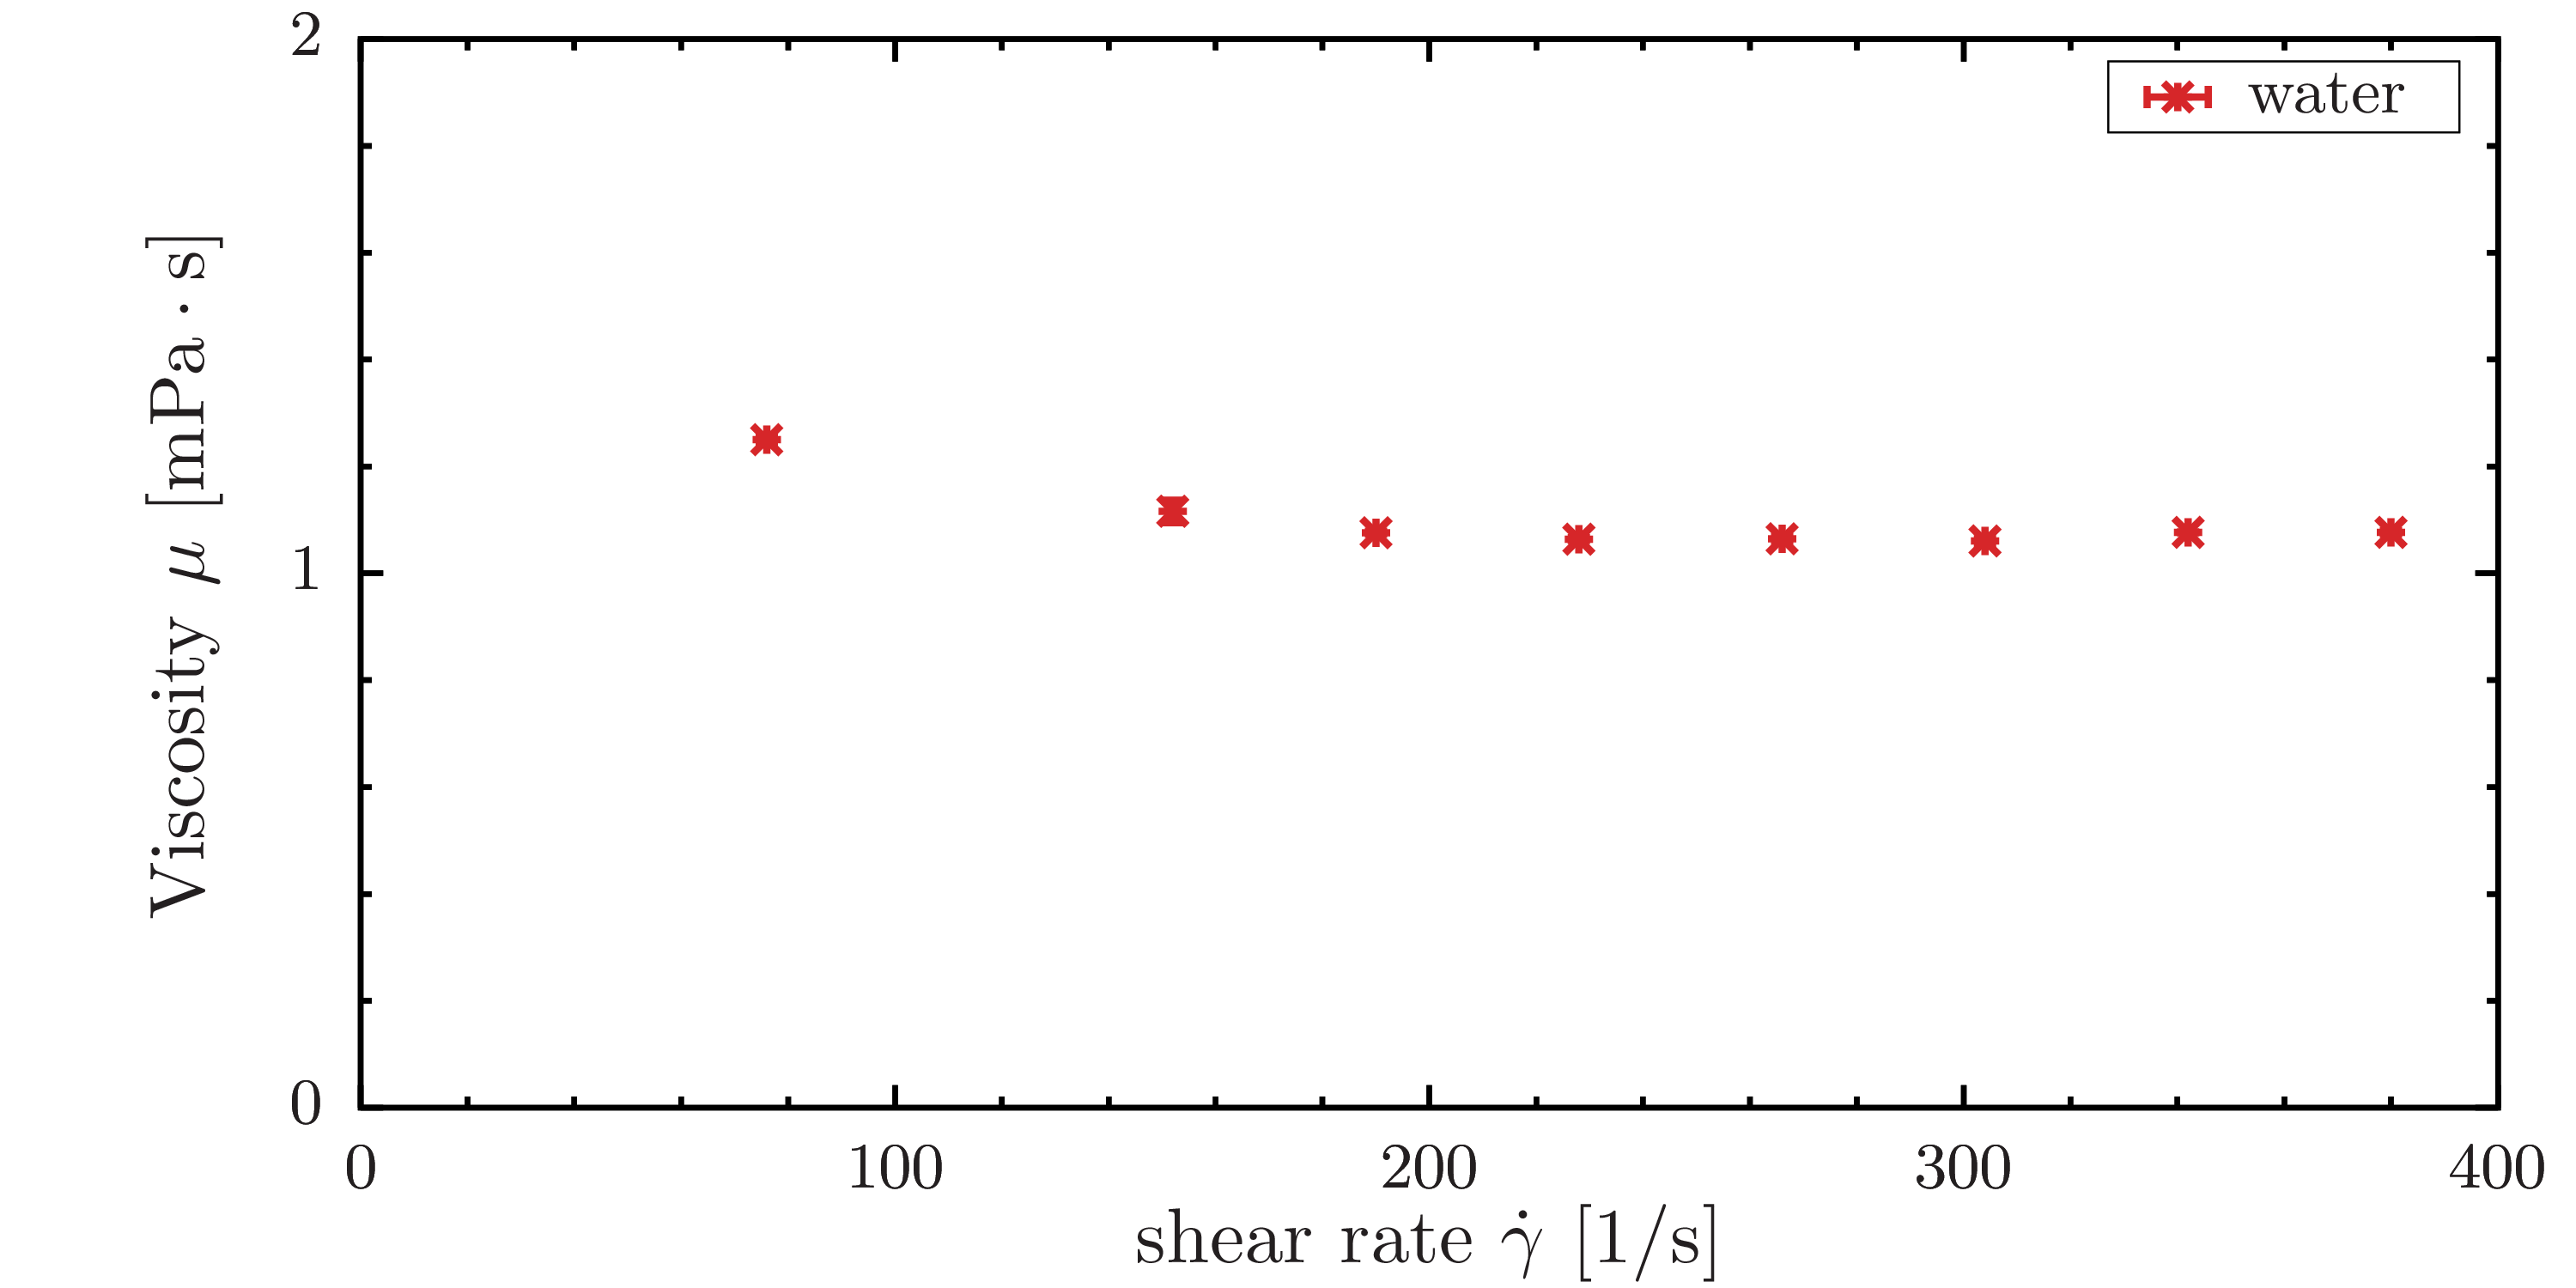
\includegraphics[width=12cm,clip]{4-Results/water.png}
    \caption{Meansured viscosity versus shear rate for tap water.}
    \label{fig:water-vis}
\end{figure}

\begin{figure}[ht]
    \centering
    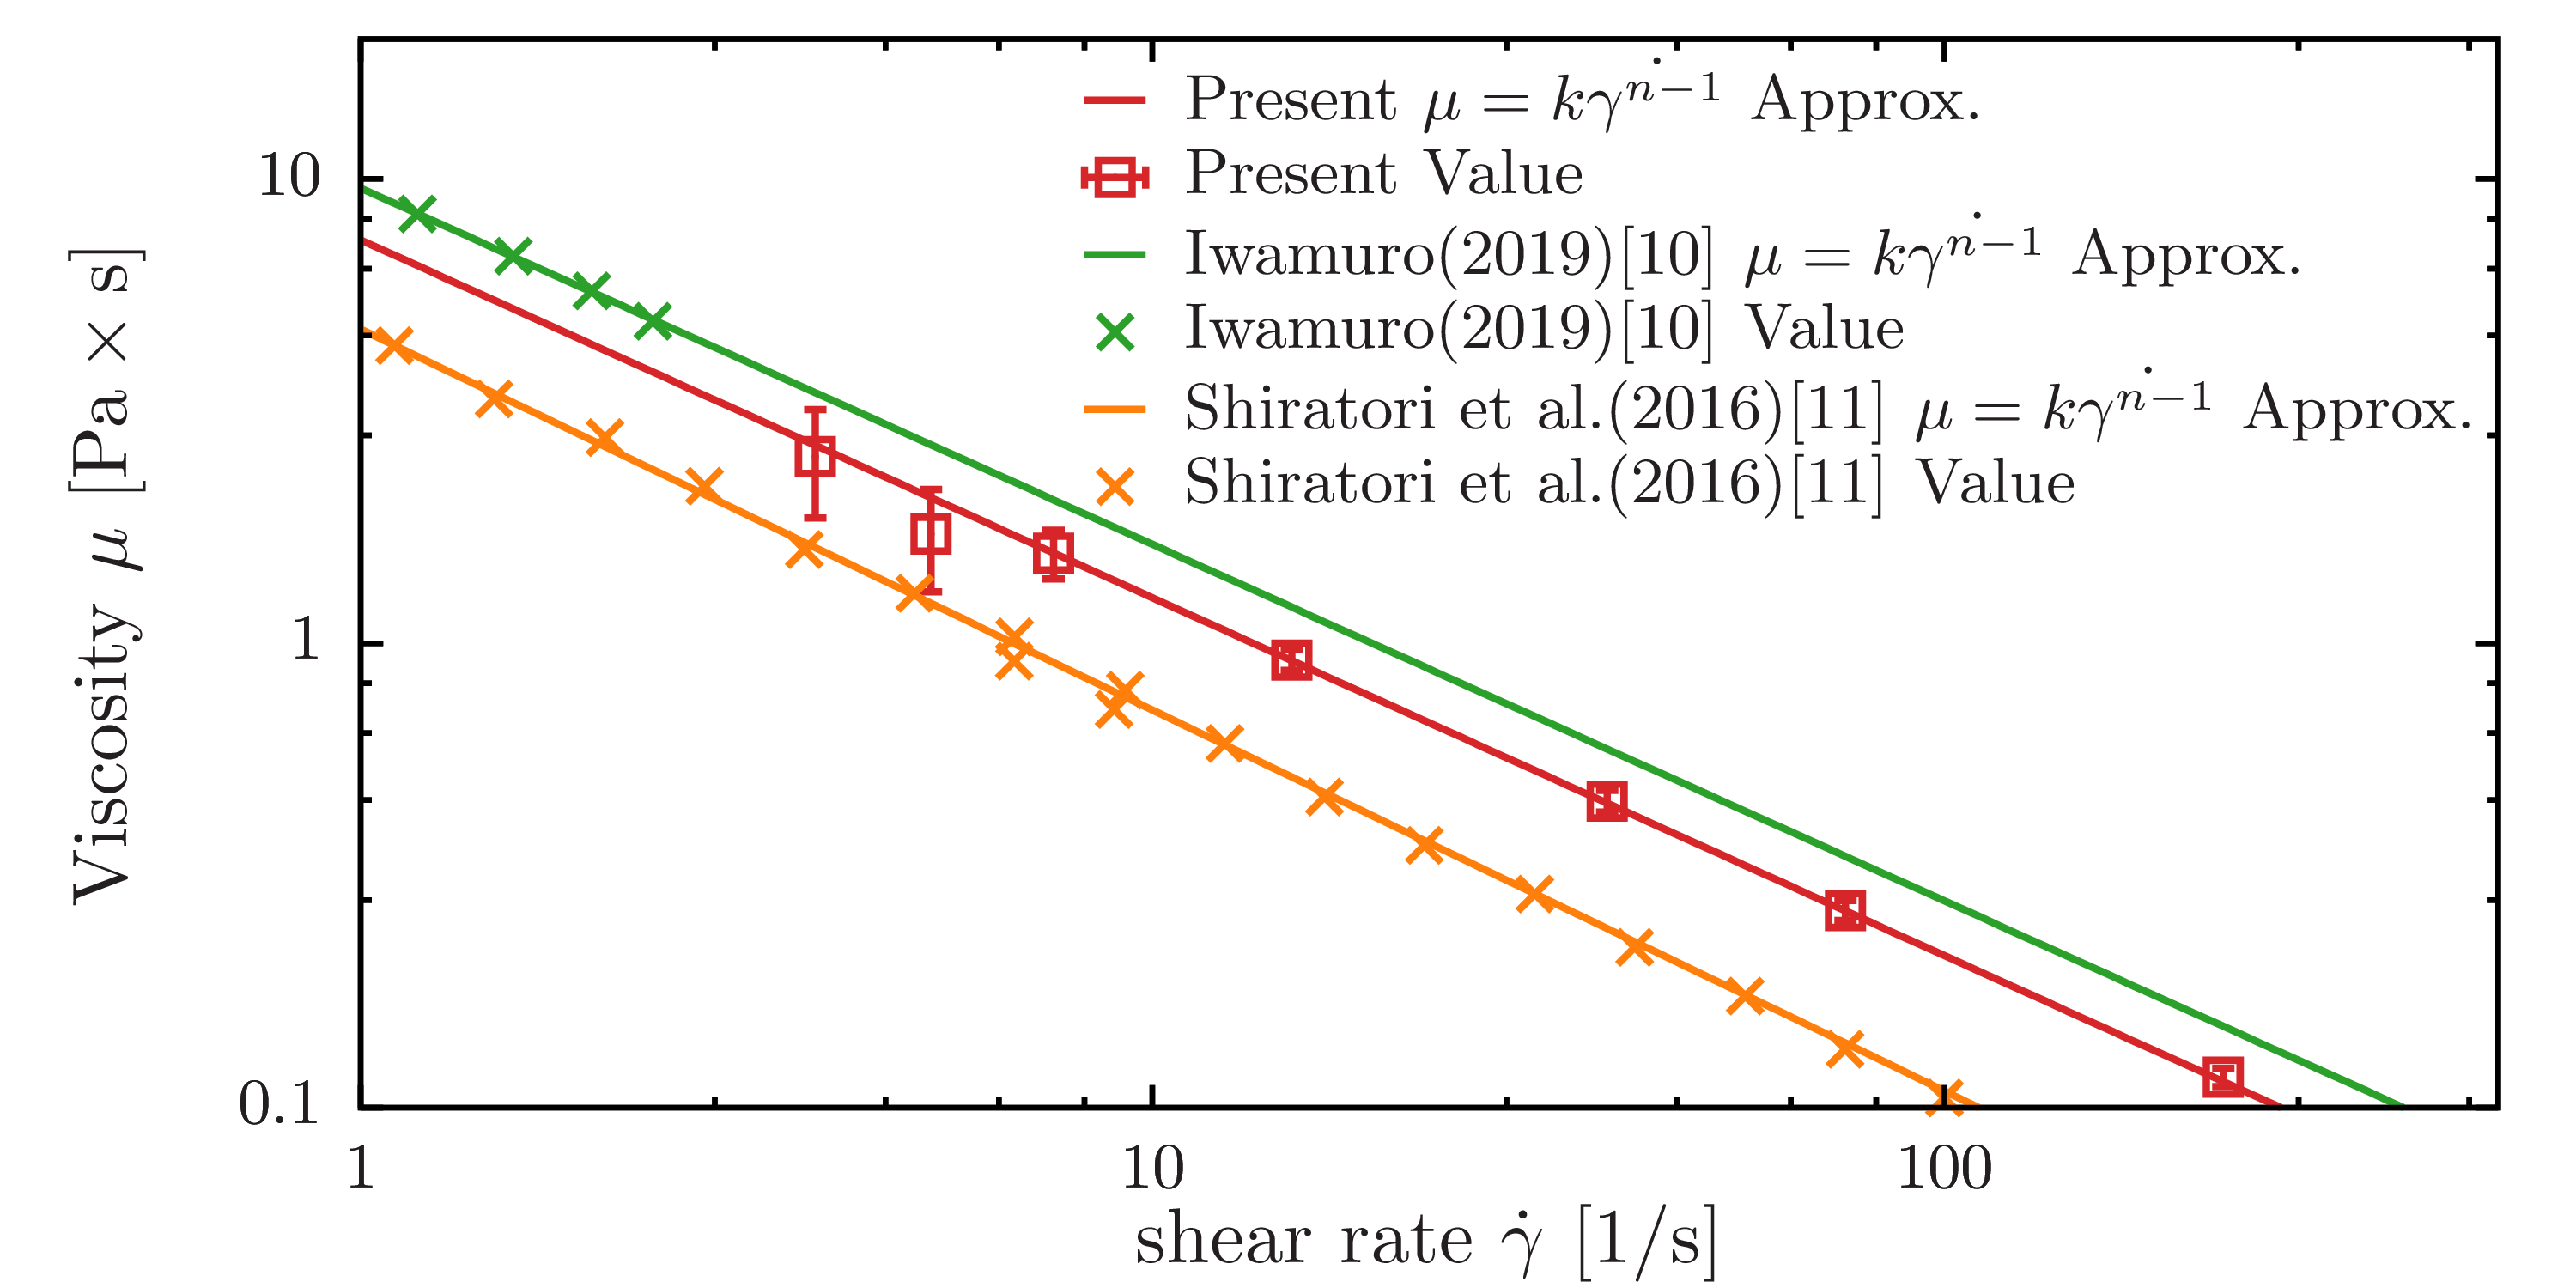
\includegraphics[width=12cm,clip]{4-Results/PAA-viscosity.png}
    \caption{Flow curve for 1wt.\%PAA solution.}
    \label{fig:PAA-vis}
\end{figure}

\newpage

\subsection{圧力場 計測結果}

圧力場の計測を行った結果をFig.\ref{fig:pressure}に示す.この結果から

\begin{figure}
    \centering
    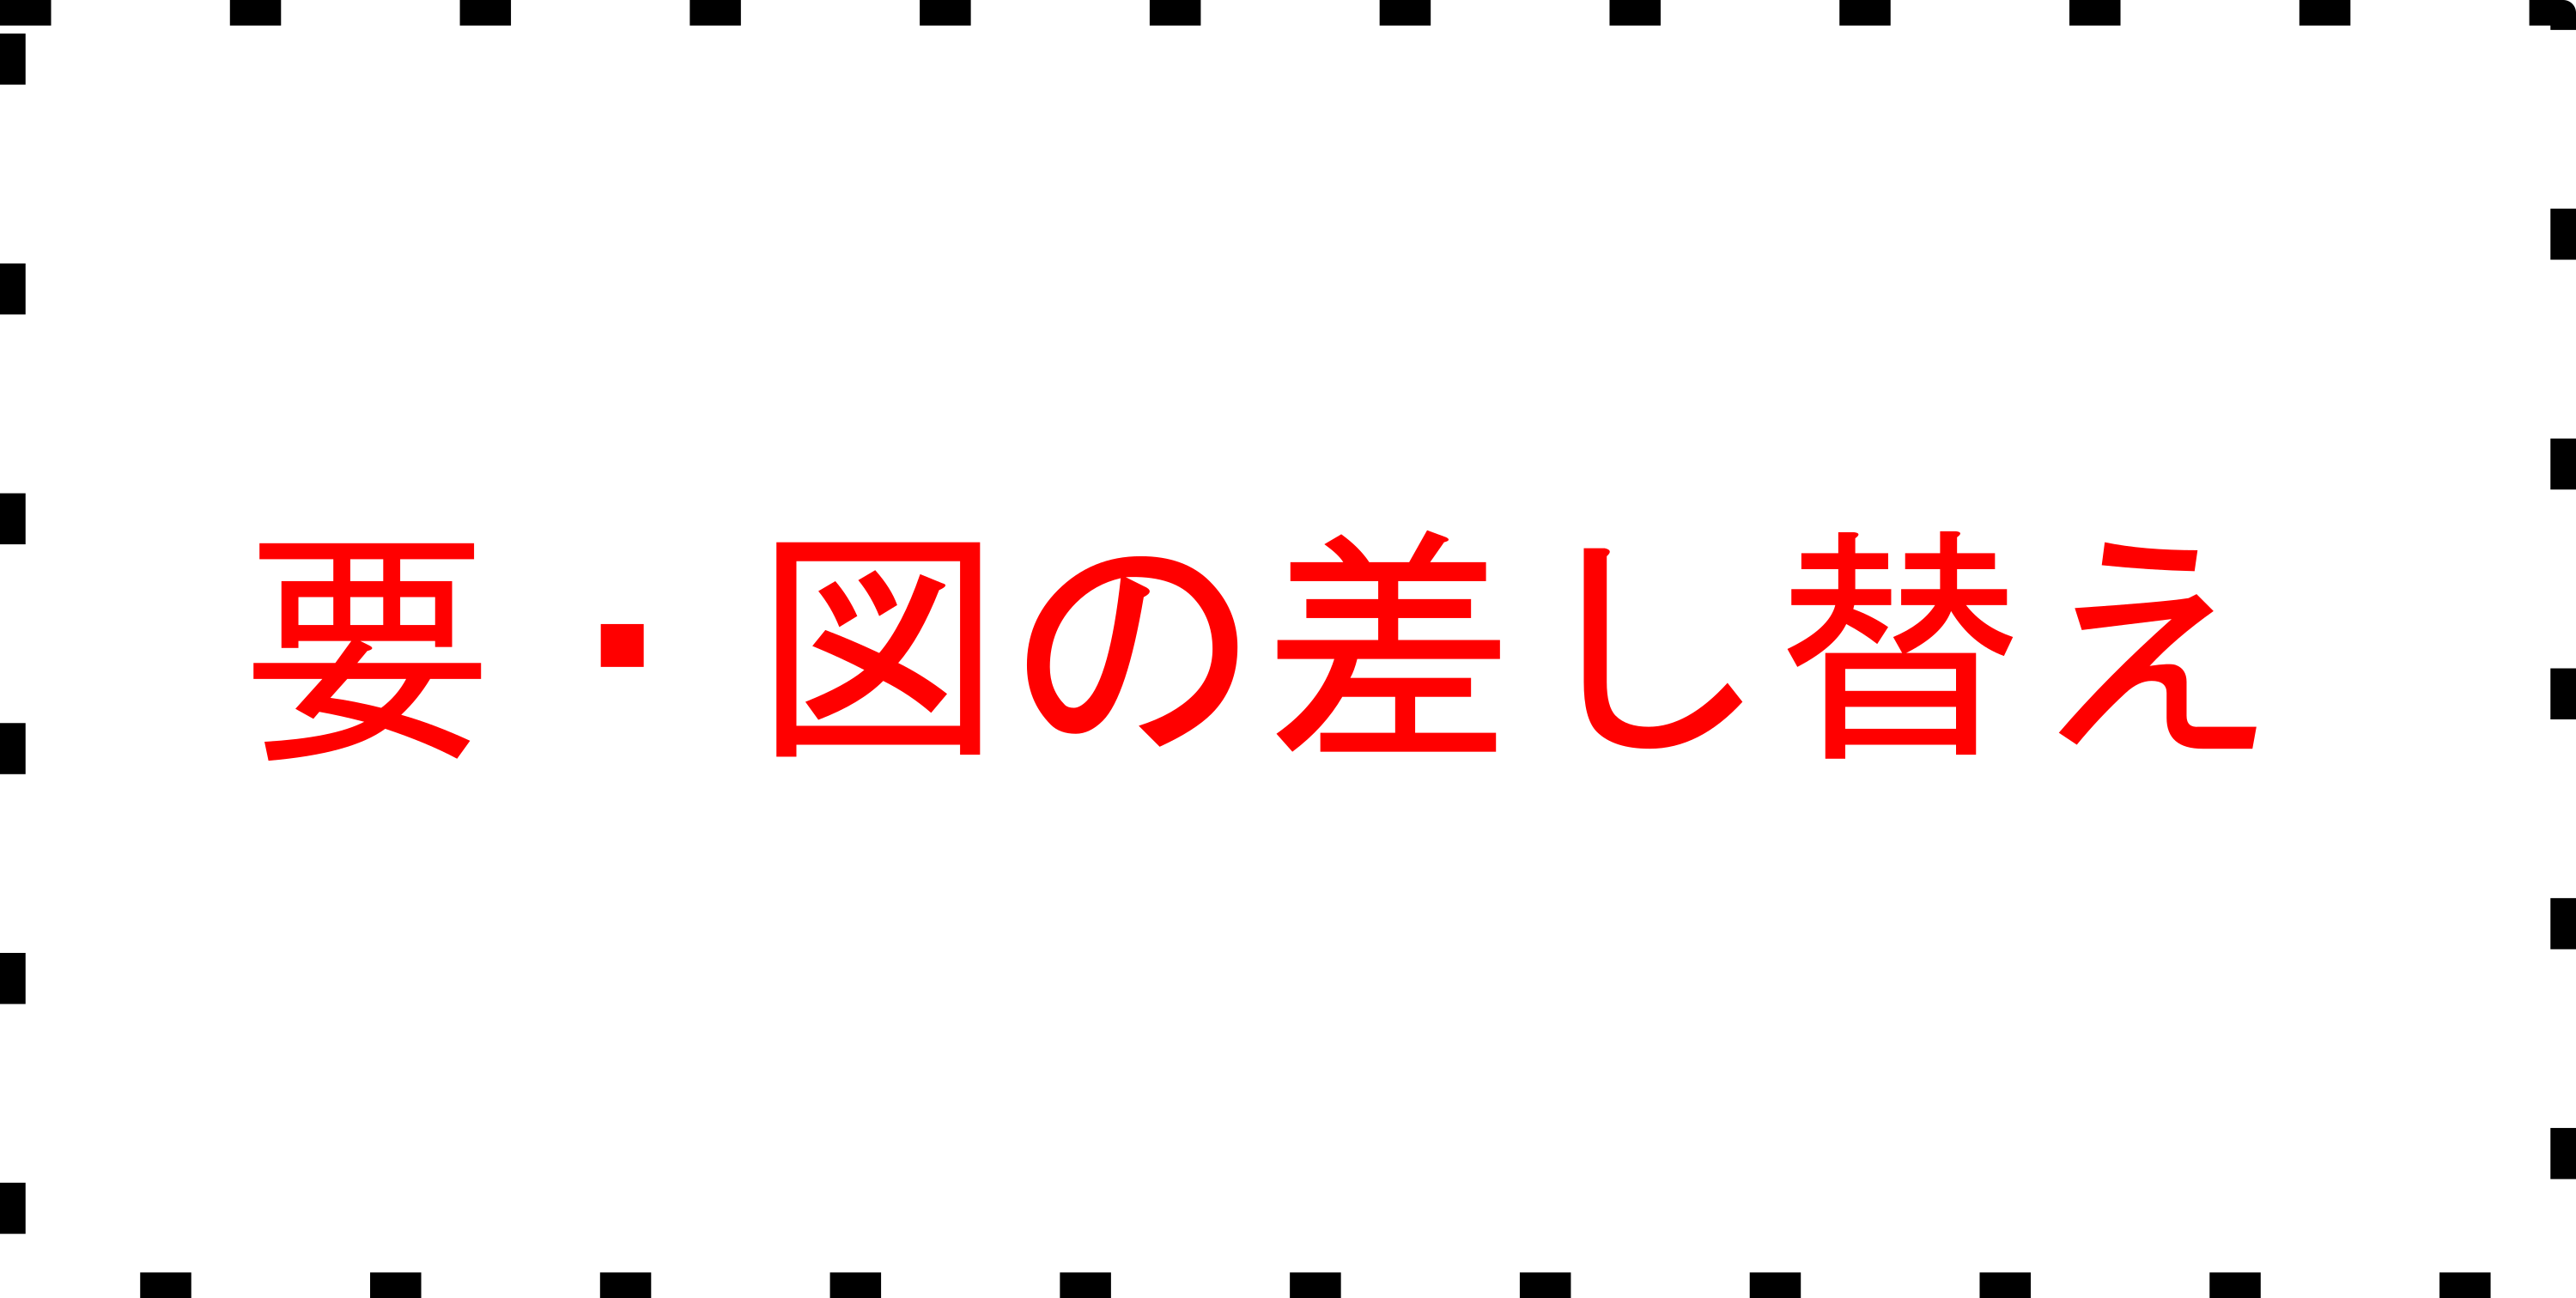
\includegraphics[width=10cm,clip]{tmp.png}
    \caption{Pressure field measurement results.}
    \label{fig:pressure}
\end{figure}

\subsection{落下球実験結果}

\begin{figure}[h]
    \centering
    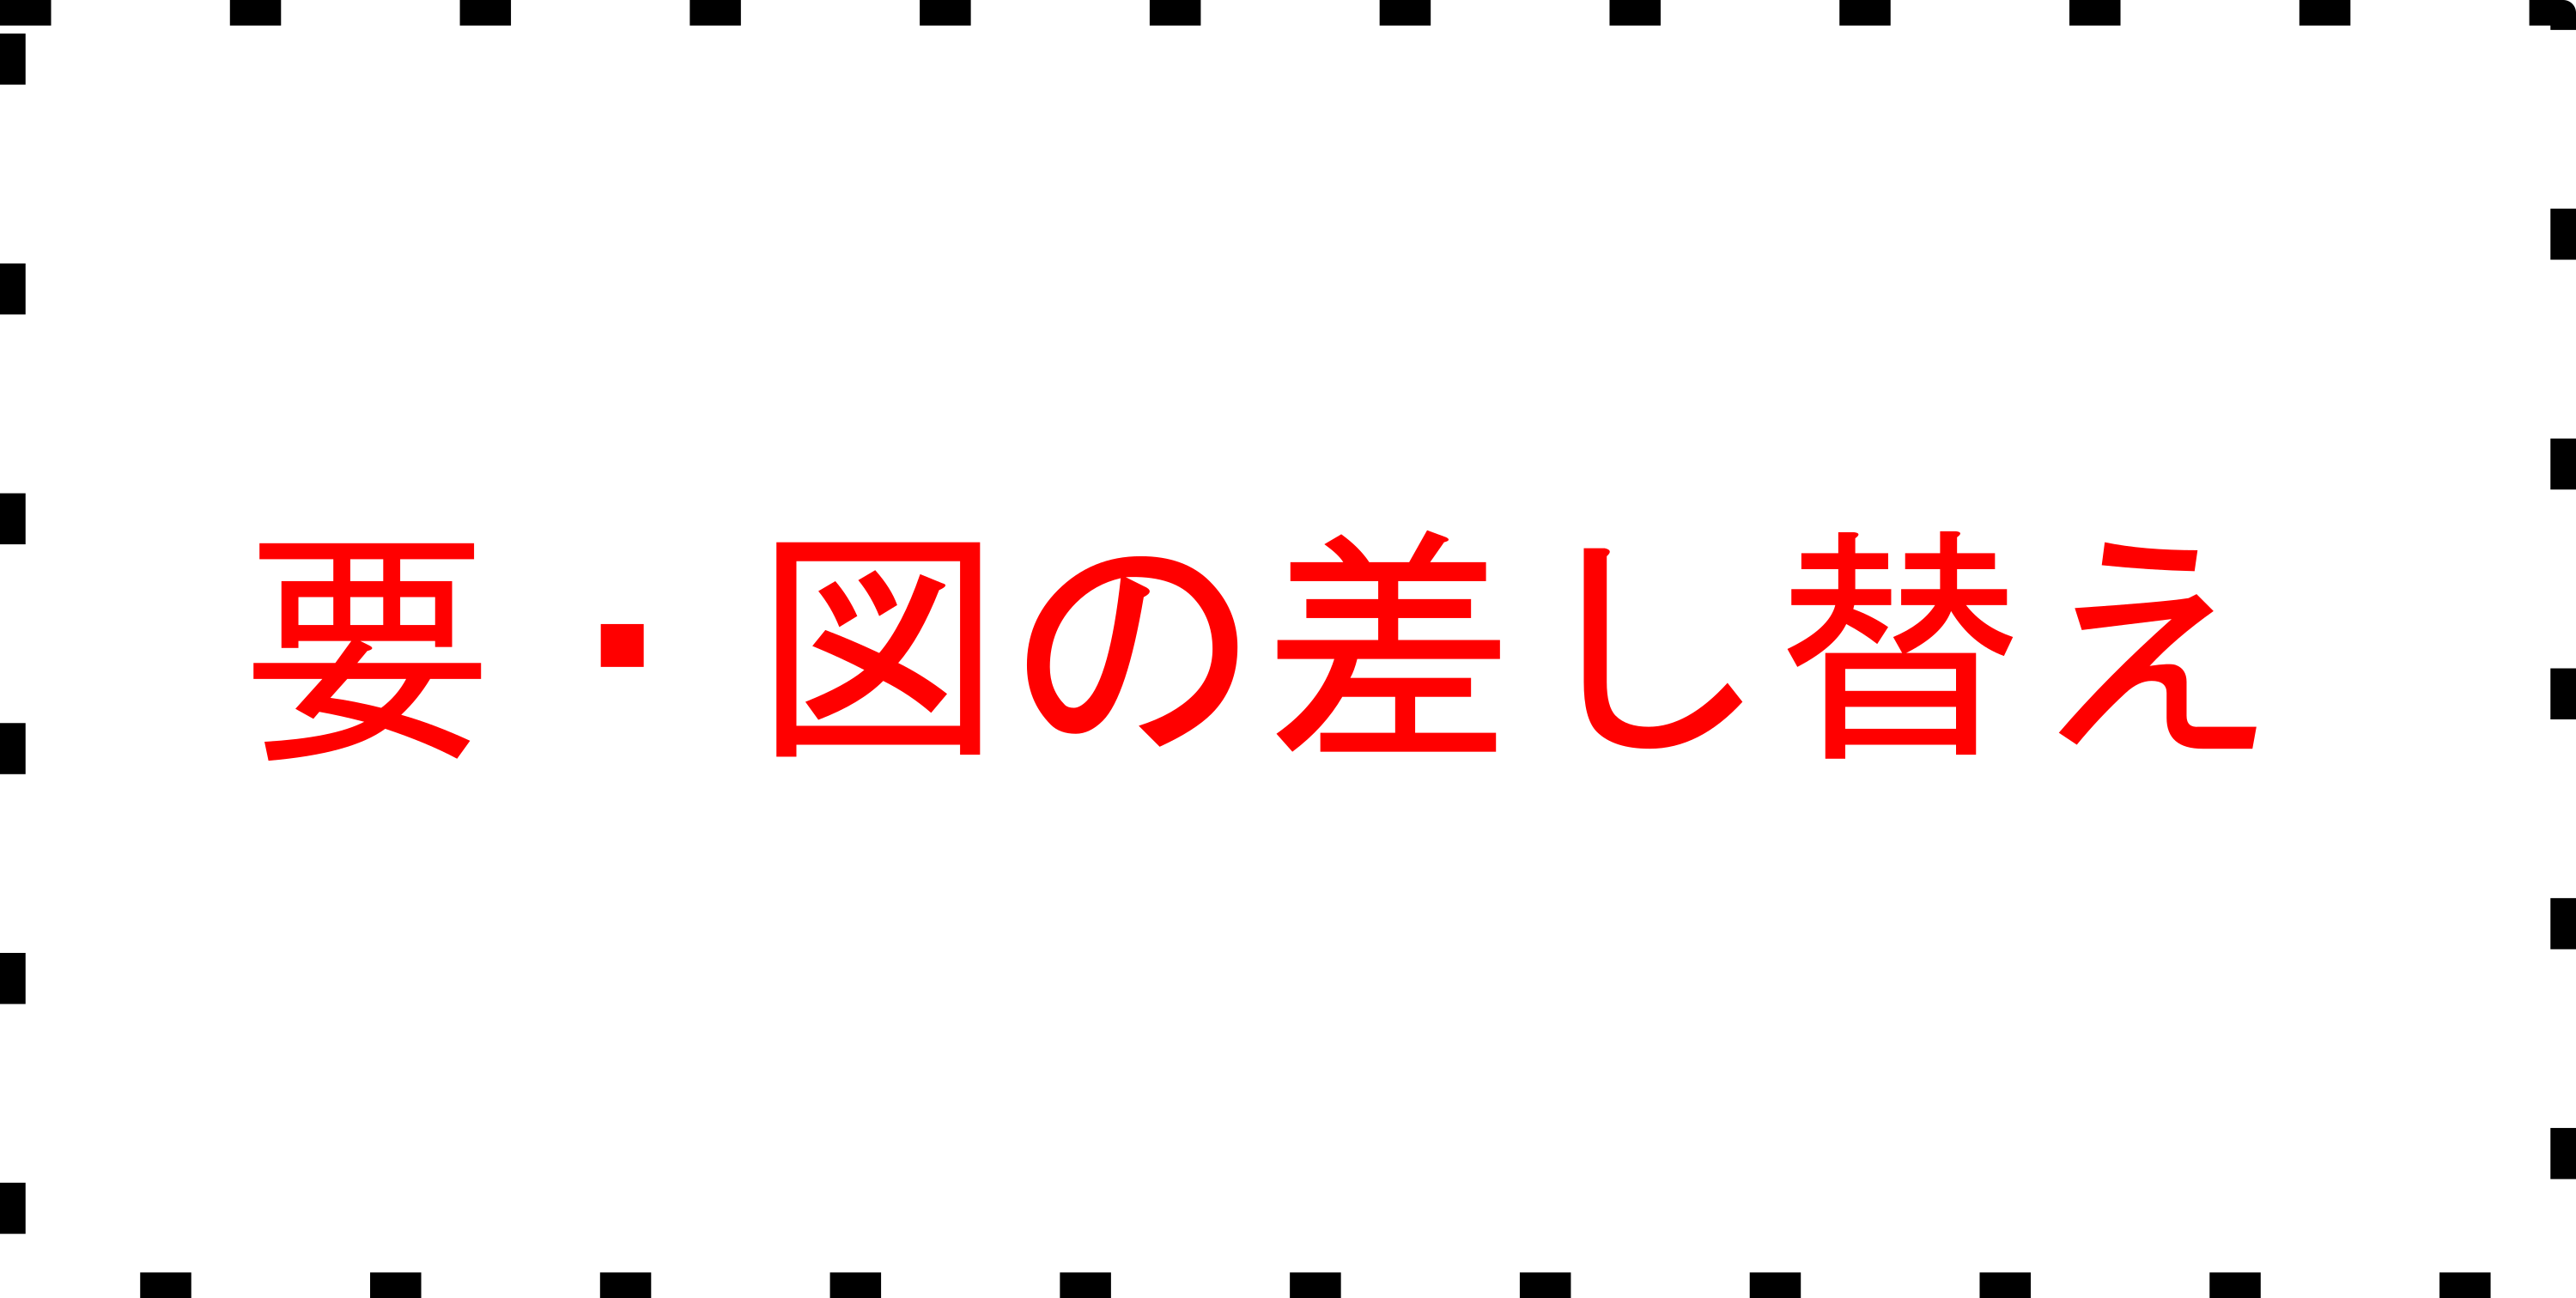
\includegraphics[width=10cm,clip]{tmp.png}
    \caption{Velocity of a falling sphere with a diameter of 2.4mm in water with or without ultrasound irradiation.}
    \label{fig:water}
\end{figure}

\begin{figure}[h]
    \centering
    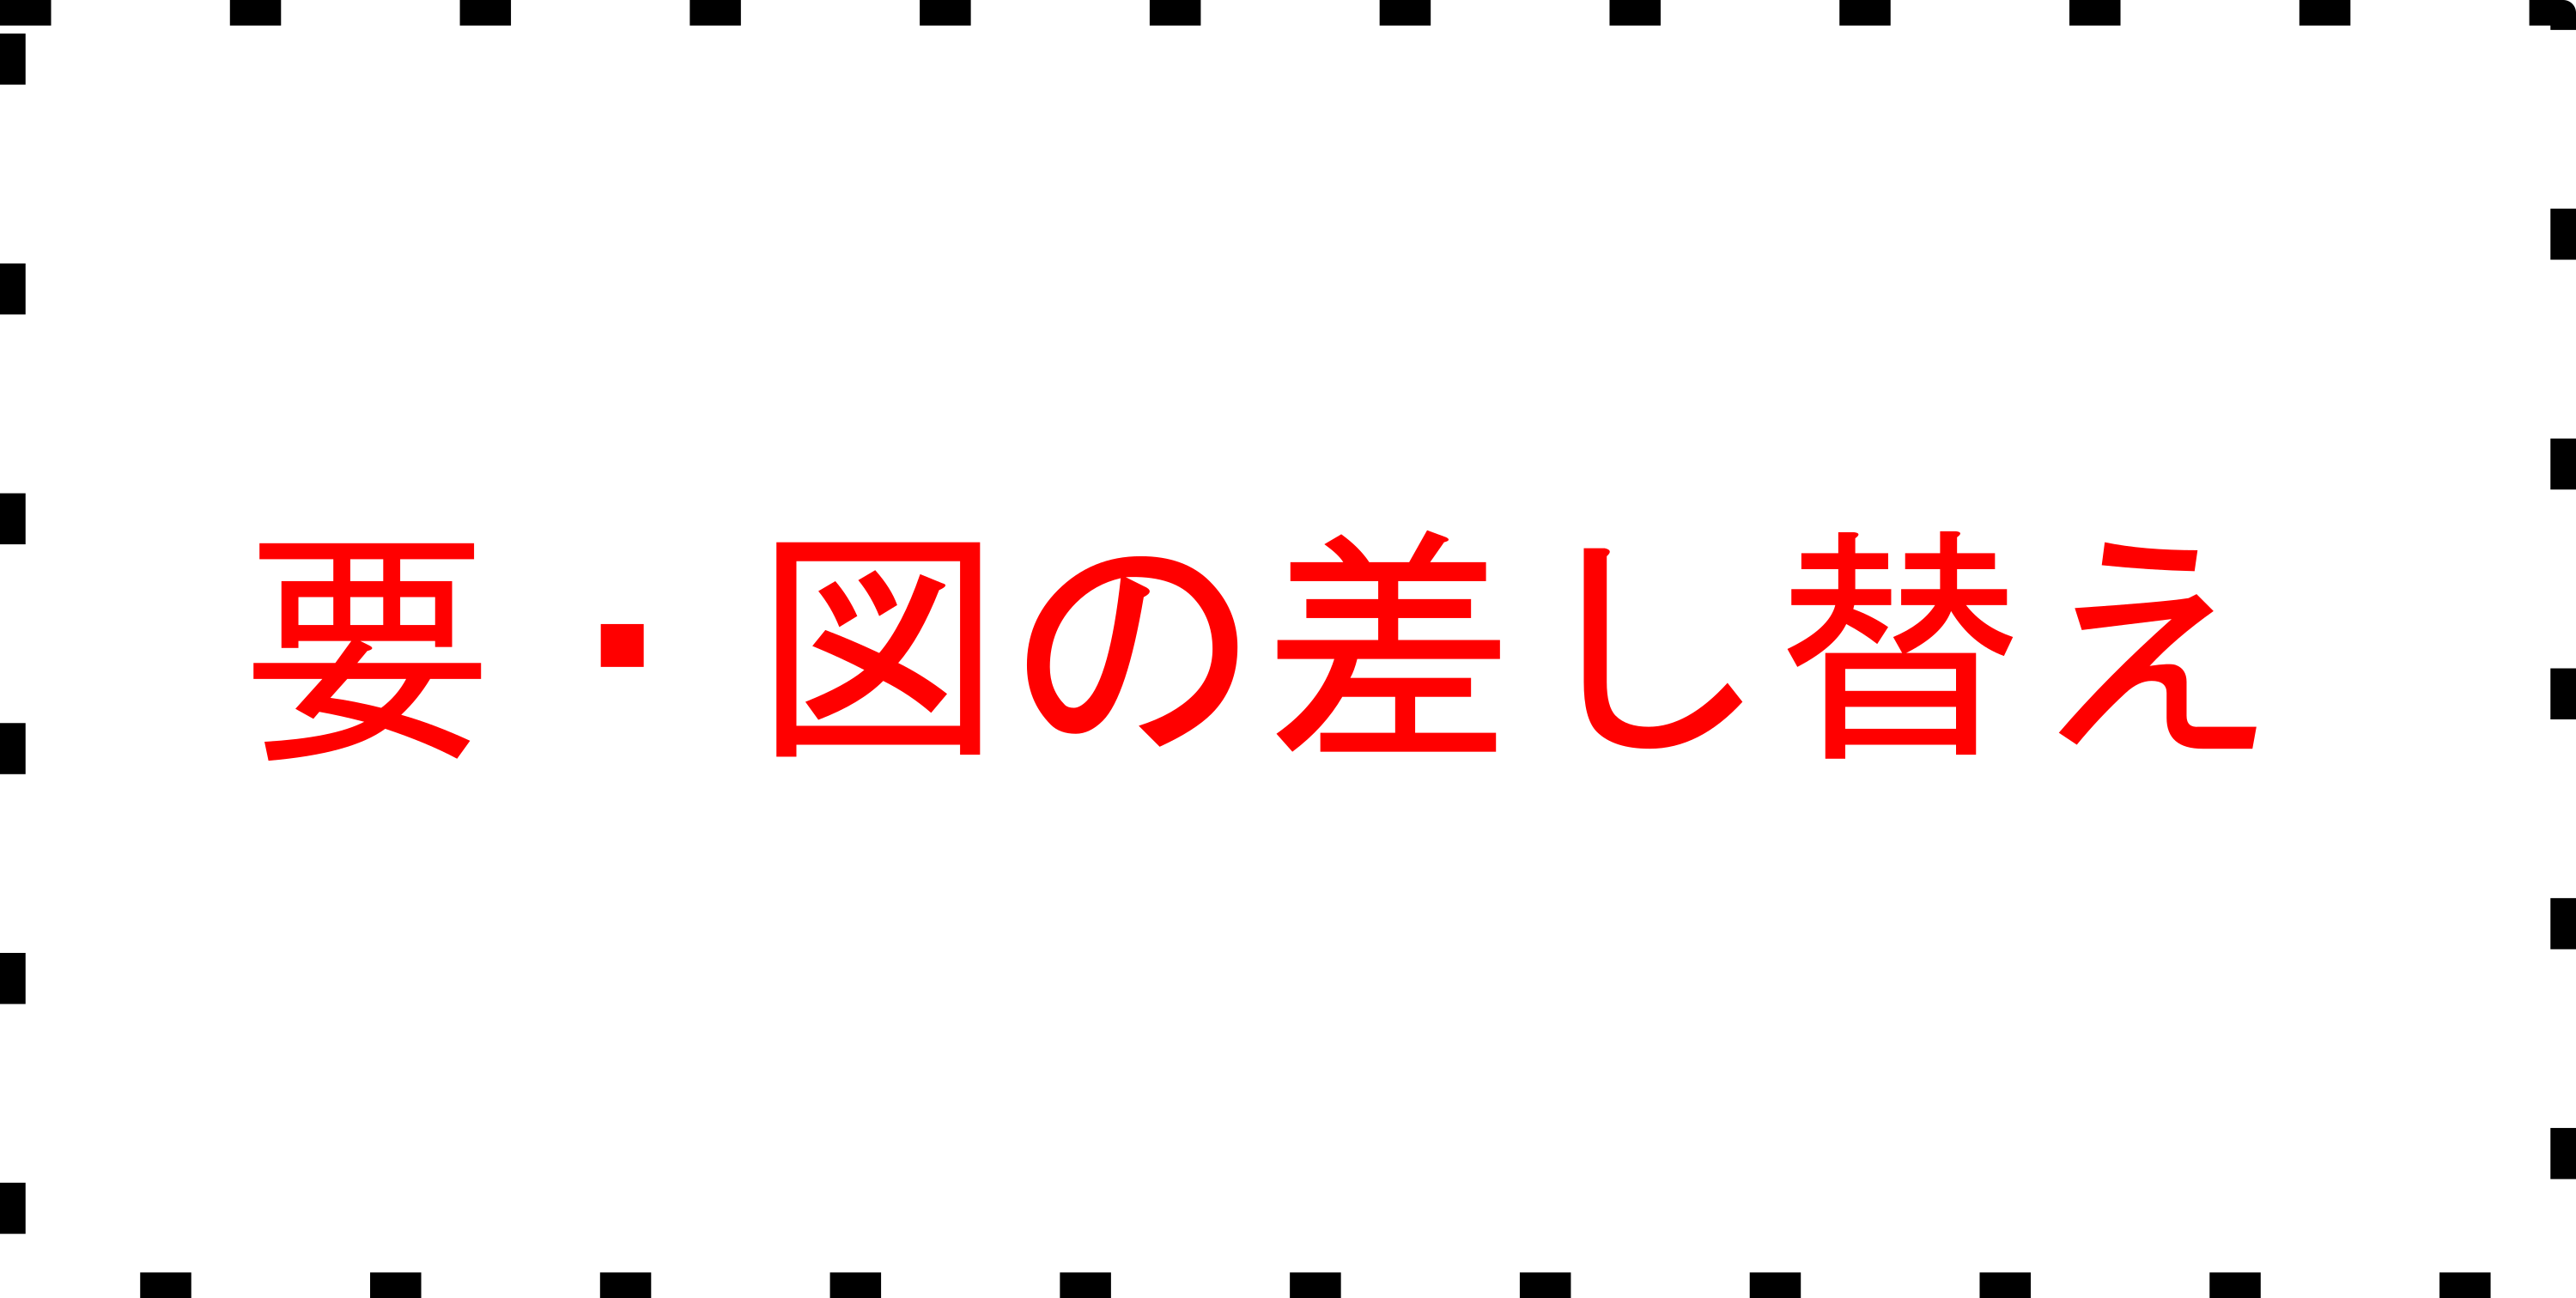
\includegraphics[width=10cm,clip]{tmp.png}
    \caption{Velocity of a falling sphere in PAA solution for various frequency of
        ultrasound irradiation.}
    \label{fig:PAA-falling}
\end{figure}
